% Options for packages loaded elsewhere
\PassOptionsToPackage{unicode}{hyperref}
\PassOptionsToPackage{hyphens}{url}
%
\documentclass[
  a4paper,
]{article}
\usepackage{amsmath,amssymb}
\usepackage{setspace}
\usepackage{iftex}
\ifPDFTeX
  \usepackage[T1]{fontenc}
  \usepackage[utf8]{inputenc}
  \usepackage{textcomp} % provide euro and other symbols
\else % if luatex or xetex
  \usepackage{unicode-math} % this also loads fontspec
  \defaultfontfeatures{Scale=MatchLowercase}
  \defaultfontfeatures[\rmfamily]{Ligatures=TeX,Scale=1}
\fi
\usepackage{lmodern}
\ifPDFTeX\else
  % xetex/luatex font selection
\fi
% Use upquote if available, for straight quotes in verbatim environments
\IfFileExists{upquote.sty}{\usepackage{upquote}}{}
\IfFileExists{microtype.sty}{% use microtype if available
  \usepackage[]{microtype}
  \UseMicrotypeSet[protrusion]{basicmath} % disable protrusion for tt fonts
}{}
\makeatletter
\@ifundefined{KOMAClassName}{% if non-KOMA class
  \IfFileExists{parskip.sty}{%
    \usepackage{parskip}
  }{% else
    \setlength{\parindent}{0pt}
    \setlength{\parskip}{6pt plus 2pt minus 1pt}}
}{% if KOMA class
  \KOMAoptions{parskip=half}}
\makeatother
\usepackage{xcolor}
\usepackage[margin=1in]{geometry}
\usepackage{graphicx}
\makeatletter
\def\maxwidth{\ifdim\Gin@nat@width>\linewidth\linewidth\else\Gin@nat@width\fi}
\def\maxheight{\ifdim\Gin@nat@height>\textheight\textheight\else\Gin@nat@height\fi}
\makeatother
% Scale images if necessary, so that they will not overflow the page
% margins by default, and it is still possible to overwrite the defaults
% using explicit options in \includegraphics[width, height, ...]{}
\setkeys{Gin}{width=\maxwidth,height=\maxheight,keepaspectratio}
% Set default figure placement to htbp
\makeatletter
\def\fps@figure{htbp}
\makeatother
\setlength{\emergencystretch}{3em} % prevent overfull lines
\providecommand{\tightlist}{%
  \setlength{\itemsep}{0pt}\setlength{\parskip}{0pt}}
\setcounter{secnumdepth}{-\maxdimen} % remove section numbering
\ifLuaTeX
\usepackage[bidi=basic]{babel}
\else
\usepackage[bidi=default]{babel}
\fi
\babelprovide[main,import]{catalan}
% get rid of language-specific shorthands (see #6817):
\let\LanguageShortHands\languageshorthands
\def\languageshorthands#1{}
\ifLuaTeX
  \usepackage{selnolig}  % disable illegal ligatures
\fi
\usepackage{bookmark}
\IfFileExists{xurl.sty}{\usepackage{xurl}}{} % add URL line breaks if available
\urlstyle{same}
\hypersetup{
  pdftitle={U3. WINDOWS SERVER. ADMINISTRACIÓ I CONFIGURACIÓ (V)},
  pdfauthor={@tofermos 2024},
  pdflang={ca-ES},
  hidelinks,
  pdfcreator={LaTeX via pandoc}}

\title{U3. WINDOWS SERVER. ADMINISTRACIÓ I CONFIGURACIÓ (V)}
\usepackage{etoolbox}
\makeatletter
\providecommand{\subtitle}[1]{% add subtitle to \maketitle
  \apptocmd{\@title}{\par {\large #1 \par}}{}{}
}
\makeatother
\subtitle{GESTIÓ DE UO I AVANÇ DIRECTIVES LOCALS DE SEGURETAT}
\author{@tofermos 2024}
\date{}

\begin{document}
\maketitle

{
\setcounter{tocdepth}{2}
\tableofcontents
}
\setstretch{1.5}
\newpage
\renewcommand\tablename{Tabla}

\section{1 Les UO}\label{les-uo}

Com ja hem explicat les UO són un objecte contenidor, d'ahi que es
representa al GUI amb una icona similar a la de els carpetes. El
contigut de les UO són altres objectes: usuaris, grups, carpetes
compartides i també altres UO.

\subsection{Per a què es creen les
UO?}\label{per-a-quuxe8-es-creen-les-uo}

Les UO són transparents a l'usuari. Un comptable pot detectar que forma
part d'alguna ``agrupació'' de companys del mateix despatx o continus i
intuir que són un ``grup'' d'usuaris. Però li costaria més intuir o
deduir la existència de UOs. De mode simplificat podríem dir que les UO
es creen per administrar la xarxa per parts. Per a que els
adminstradors, o usuaris avançats habilitats, puguen repartir-se la
faena d'administrar la xarxa sencera.

Els criteris o raons per crear UO poden ser tres:

1- Dividir l'administració del domini atenent a un \textbf{criteri
geogràfic}. Delegacions de països, zones\ldots{} o centres d producció
distints. 2- Dividir l'administració del domini atenent a un
\textbf{criteri organitzatiu}. Agrupant departaments de l'empresa, per
exemple. 3- Crear agrupacions d'objectes de forma \textbf{dinàmica} per
a projectes temporals. Una UO amb tots els recursos (objetes) per crear
una aplicació software nova, per desenvolupar un prjecte
urbanístics\ldots{}

\subsection{La divisió del treball duu
l'especialització}\label{la-divisiuxf3-del-treball-duu-lespecialitzaciuxf3}

El que està clar és que abandonem el paradigam de l'\emph{administrador
o administradors de tot el domini} i obrim les portes a que un usuari
(no necessàriament administrador) puga fer tasques (encara que bàsiques)
en el Servidor pròpies d'un administrador.

\section{2 La delegació de control de la
UO}\label{la-delegaciuxf3-de-control-de-la-uo}

Ja hem vist en aquesta unitat (U3.2) com es creen les UO i com es
modifiquen. Ara vorem com es delega el control en un usuari. Delegar el
control en un usuari Administrador del domini pot semblar un poc absurd;
interessa delegar en un altre tipus d'usuari que no siga Administrador
del tot per a convertir-lo en un ``quasi-administrador'' d'una part del
domini (la UO).

\subsection{2.1 Selecionem l'usuari, usuaris o
grups}\label{selecionem-lusuari-usuaris-o-grups}

En el nostre exemple triarem un usuari \emph{jefeNord} per a la
\emph{UO-DelegacióNord}.

Hem de buscar i seleccionar correctament l'usuari.

\begin{figure}
\centering
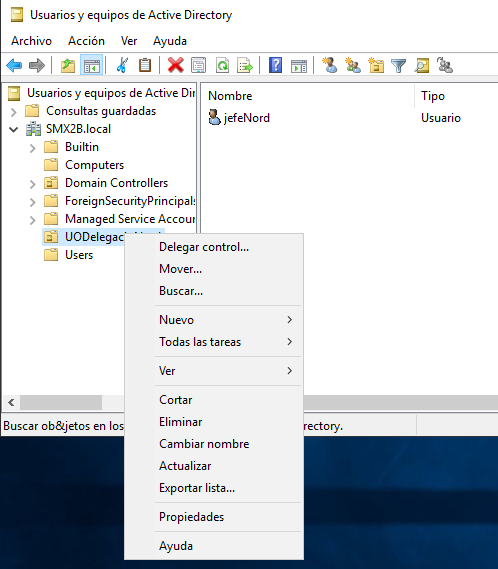
\includegraphics{png/DelegarControl1.png}
\caption{\emph{Figura 1:Delegar control}}
\end{figure}

\subsection{2.2 Assignem drets}\label{assignem-drets}

\begin{figure}
\centering
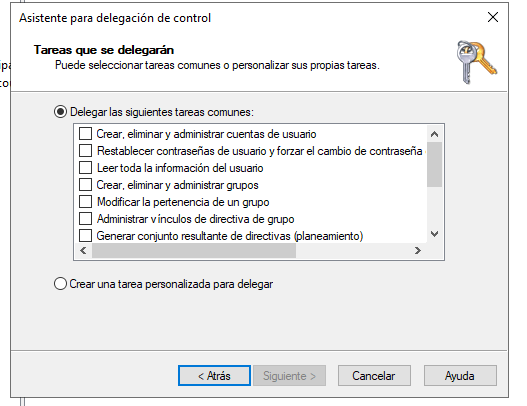
\includegraphics{png/DelegarControl2.png}
\caption{\emph{Figura 2: Assignar drets en la delegació}}
\end{figure}

Un exemple d'ús senzill és d'autoritzar a un usuari de la Delegació,
Centre de Producció o Projecte que represente la UO per a que reinicie
les contrassenyes dels usuaris. Així cada vegada que un operador
d'ordinador se li oblida la contrasenya no cal que cride a
l'administrador

\begin{quote}
Nota:

Fixem-nos en el detall que parlem de ``drets'' i no de ``permisos'' que
és un terme que circumscriurem a l'ambit del sistema de fitxers.
\end{quote}

\subsection{2.3 Habilitem l'usuari per a iniciar
sessió.}\label{habilitem-lusuari-per-a-iniciar-sessiuxf3.}

Com bé sabem, els grups d'usuaris que poden iniciar sessió al servidor
per defecte, en acabar la instal·lació de Windows Server, són alguns
grups predeterminats que direm genèricament i mal dit ``administradors''
(Administradors del servidor, del domini, operadors de comptes\ldots).
Té la seua raó en la seguretat evidentment.

\begin{figure}
\centering
\includegraphics{png/usuarisDEfecteWS.png}
\caption{Figura 3:Usuaris per defecte}
\end{figure}

Com ja hem exposat, ara, anem a fer una excepció permentent l'accés al
servidor a un usuari del domini (no és un informàtic dedicat a
l'administració de la LAN) per a que faça només \textbf{estrictament}
les accions que hem especificat adés com a drets.

A la \emph{Unitat 5. Windows Server. Monitorització i ús} tractarem
l'inici de sessió remota, ara farem l'inici local.

\textbf{Spoiler: directiva de seguretat}

Tot i que les Directives de Seguretat es tracten a la \emph{Unitat
4.Administració i configuració avançada} s'imposa la necessitat de fer
un spoiler.

\subsubsection{\texorpdfstring{Canvi de la directiva: ``Permitir inicio
en sesión
local''''}{Canvi de la directiva: ``Permitir inicio en sesión local''\,''}}\label{canvi-de-la-directiva-permitir-inicio-en-sesiuxf3n-local}

1- Executar \textbf{gpmc.msc}

\emph{A la Unitat 4 tractem un poc més a fons les directives en general}

Busquem una directiva que afecta a la màquina (\textbf{Domain
Controller}) ja que es tracta de permetre iniciar sessió local, per tant
modificarem la plantilla de directives que ve per defecte de
\textbf{Default Domain Controller Policy} la directiva: \textbf{Permitir
el inicio de sesión local}

\begin{itemize}
\item
  Observem quins grups poden inciar sessió localment en aquesta màquina.
  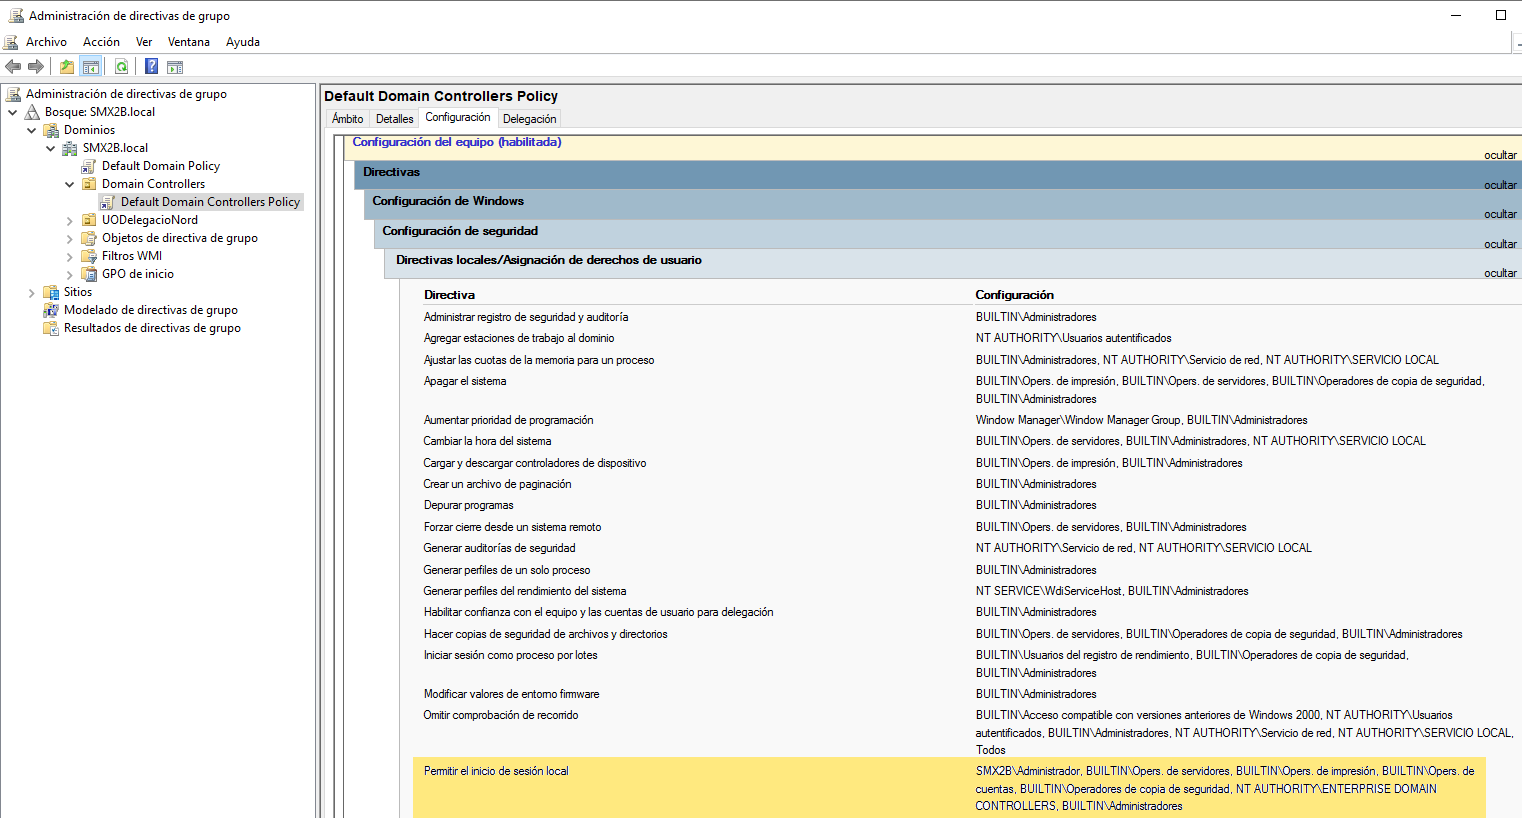
\includegraphics{png/mostrarDirectiva1.png}
\item
  Botó contrari:\textbf{EDITAR}
\end{itemize}

\begin{figure}
\centering
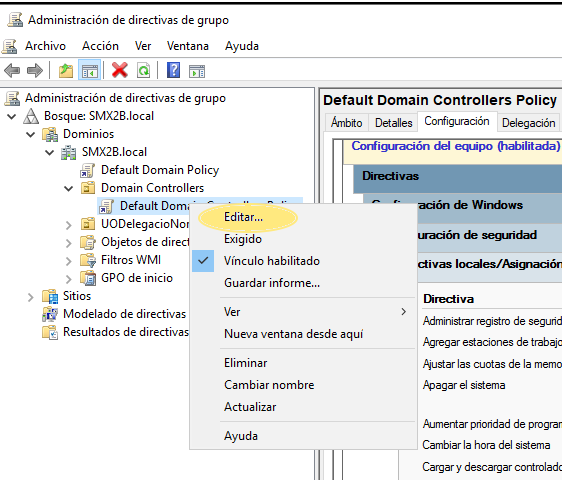
\includegraphics{png/EditarDirectiva1.png}
\caption{\emph{Figura 5:Edició de la directiva local de seguretat}}
\end{figure}

\begin{itemize}
\tightlist
\item
  Seleccionem la directiva que volem canviar
\end{itemize}

\begin{figure}
\centering
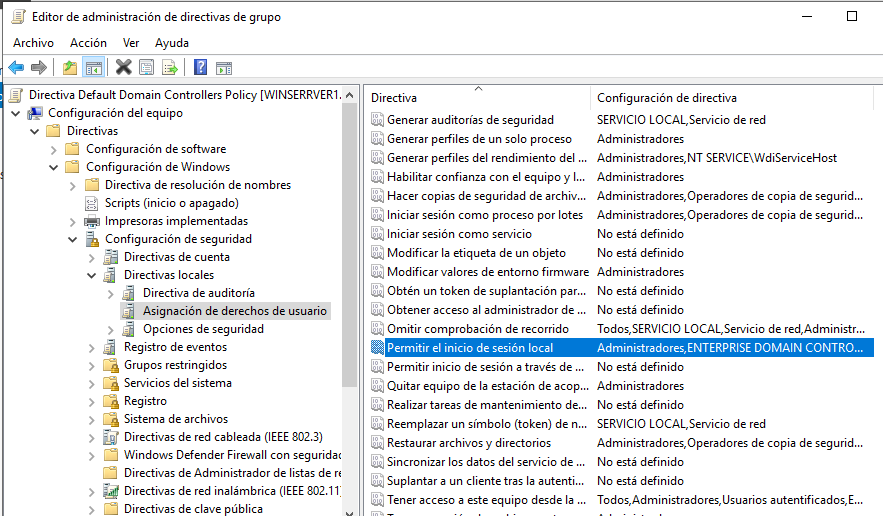
\includegraphics{png/EditarDirectiva2.png}
\caption{\emph{Figura 6:Edició de la directiva local de seguretat}}
\end{figure}

\begin{itemize}
\tightlist
\item
  Afegim l'usuari
\end{itemize}

\begin{figure}
\centering
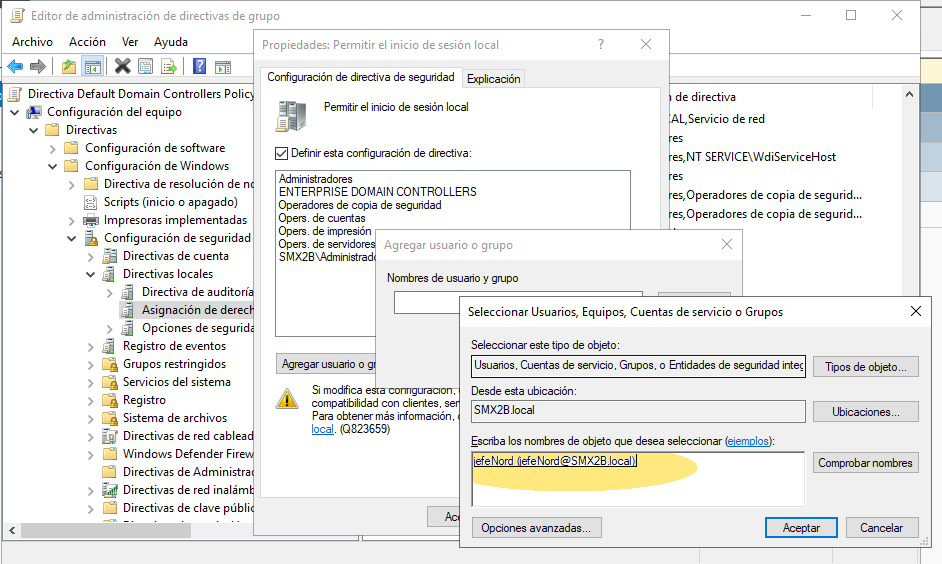
\includegraphics{png/EditarDirectiva3.png}
\caption{\emph{Figura 7:Edició de la directiva local de seguretat}}
\end{figure}

\begin{itemize}
\tightlist
\item
  Sempre que teniu \textbf{APLICAR} recordeu polsar abans que
  \textbf{Acceptar}
\end{itemize}

\begin{figure}
\centering
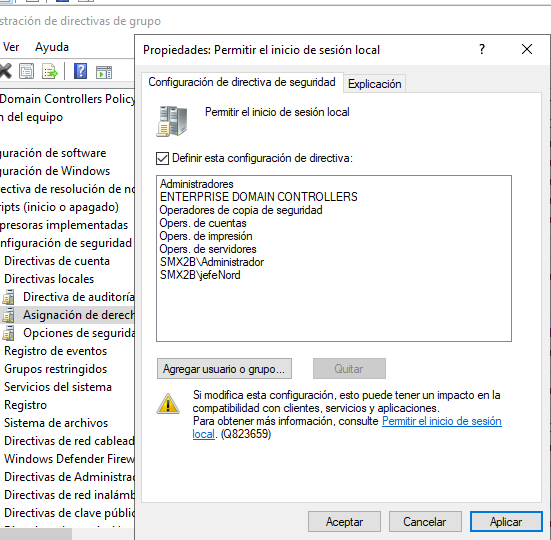
\includegraphics{png/EditarDirectiva4.png}
\caption{\emph{Figura 8:Edició de la directiva local de seguretat}}
\end{figure}

\textbf{Comprovem\ldots{}} Provem tancar la sessió de l'administrador en
ús i comprovar que l'usuari ja pot inciar sessió localment al servidor.
Efectivament, pot.

\subsection{2.4 Comprovació de les accions que podem
fer}\label{comprovaciuxf3-de-les-accions-que-podem-fer}

Per defecte, no se'ns obri el panel d'Administració de Servidor. Cosa
lògica si entenem que no som Administradors ni del servidor (local) ni
del domini.

\subsubsection{Accés a eines
d'administració}\label{accuxe9s-a-eines-dadministraciuxf3}

Si intentem accedir a alguna eina d'administració com les consoles de
Microsoft (dsa.mmc, per exmple), l'administrador del servidor
(servermanger.exe), panel de control per fer un canvi\ldots{} Ens
demanarà que ens autentiquem\ldots{}

\begin{figure}
\centering
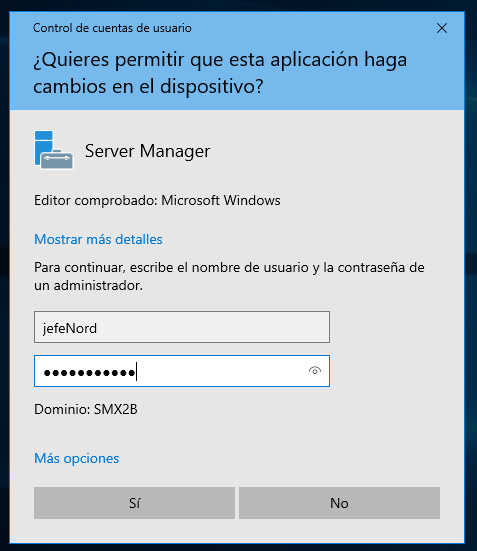
\includegraphics{png/permisUsuariDelegat.png}
\caption{\emph{Figura 3:Autenticació d'usuari}}
\end{figure}

Una vegada ens autentiquem com a l'usuari delegat veiem que podem entrar
sense problemes (en principi). És més, encara que l'acció no estava
entre les autoritzades (apartat 2.2 i Figura 2), potser ens deixe
``iniciar-la'', fer com uns ``primers pasos'' dins de cada eina GUI però
arriba un moment en que se'ns denega.

\begin{figure}
\centering
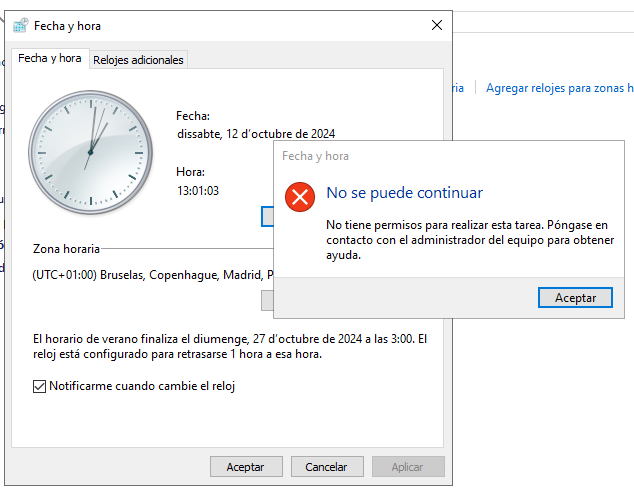
\includegraphics{png/canviHoraNO.png}
\caption{\emph{Figura 4:Panel de control, canviar hora}}
\end{figure}

\begin{figure}
\centering
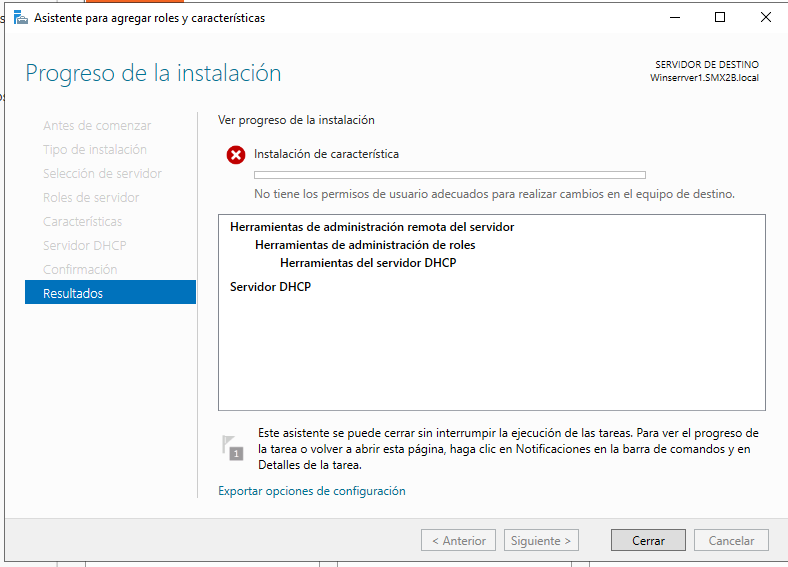
\includegraphics{png/InstalarRolNO.png}
\caption{\emph{Figura 5:Instal·lar ROL}}
\end{figure}

Una prova que heu de fer és la provar les accions permeses dins de la UO
on tenim delegat el control i fora.

\begin{figure}
\centering
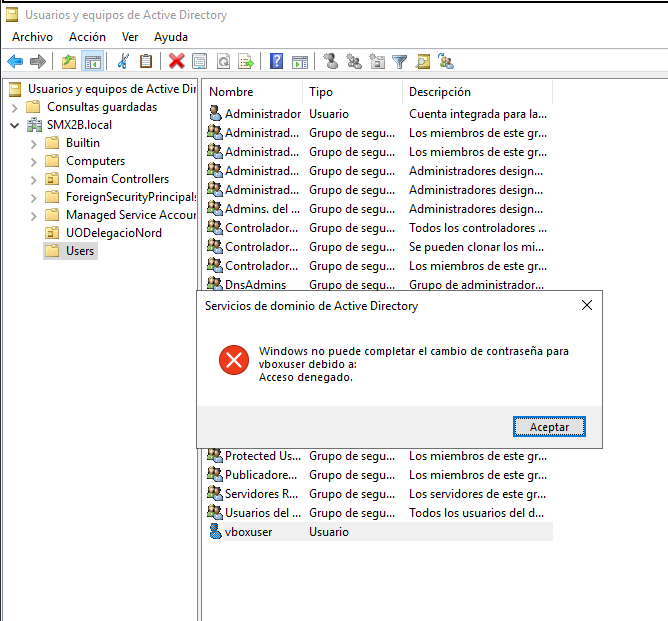
\includegraphics{png/NoTienePrivilegios.png}
\caption{\emph{Figura 6: Accions permeses però fora de la UO}}
\end{figure}

\subsection{2.5 Conclusions}\label{conclusions}

\subsubsection{Analogia i recordatori de
SOM}\label{analogia-i-recordatori-de-som}

A partir dels coneixements teòrics i pràctics del curs passat a SOM,
podem entendre què ha passat i on. El que passa és exactament el que ens
passava a l'aula de SOM, l'any anterior si, amb l'usuari d'alumne
intentàvem executar un ``sudo\ldots{}''

\textbf{Exemple 1} No podem instal·lar un ROL com quan en Linux no
podíem instal·lar un paquet\ldots{}

\begin{figure}
\centering
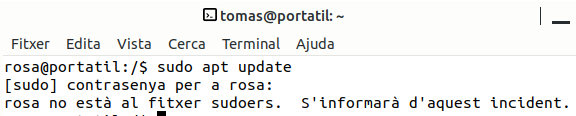
\includegraphics{png/rosaUpdate.png}
\caption{\emph{Figura 4: Eines per instal·lar apt}}
\end{figure}

\textbf{Exemple 2} No podem canviar l'hora des del Panel de Control del
Windows Server, ve a dir-nos que no ``som sudoer''

\begin{figure}
\centering
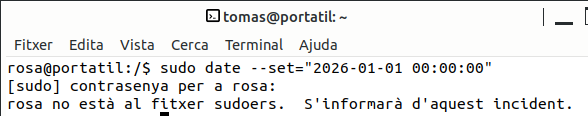
\includegraphics{png/rosaHora.png}
\caption{\emph{Figura 7: Canvi de data}}
\end{figure}

\subsubsection{Les capes del SO}\label{les-capes-del-so}

1- \textbf{Interfície usuari}

GUI: L'eina de configuració (consola msa.msc, per exemple) és un
aplicació de sistema. Hi està a la capa externa que es comunica amb
nosaltres (usuaris) i ¡, així, li donem les indicacions sobre què volem
que faça la màquina.

CLI: El terminal de Linux (o Powershell com vorem) també fan la mateixa
funció.

Relament quan ens deixa executar incialment, és com qual al terminal ens
deixa escriure ``sudo apt\ldots{}''. És quan li donem a Enter ( o
Aplicar/Acceptar) quen \textbf{enviem l'ordre al kernel} quan\ldots{}

2- \textbf{Seguretat i protecció} El Kernel (nucli del SO) de Windows i
de Linux comprovem que l'usuari no està autoritzat.

\subsubsection{Comproveu l'abast de la
delegació}\label{comproveu-labast-de-la-delegaciuxf3}

És important que comproveu que l'usuari té el control dins de la UO
estrictament. En un altra UO o a l'arrel del Domini (exemple de la
imatge següent), no.

\begin{figure}
\centering
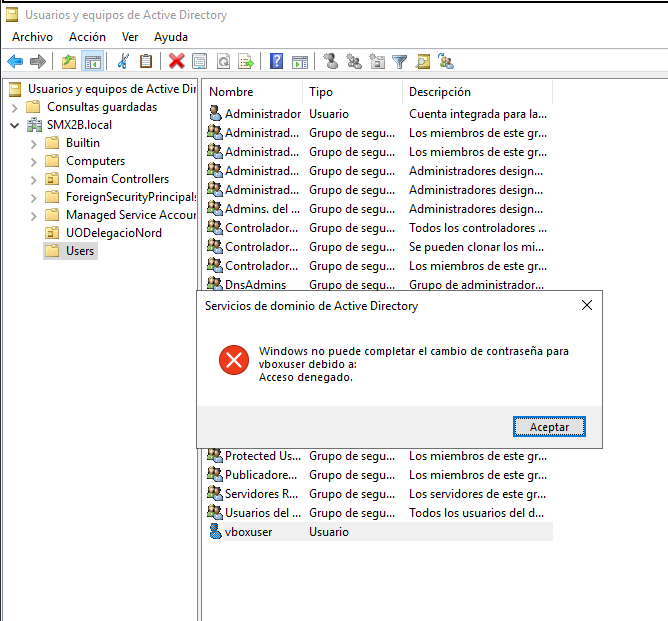
\includegraphics{png/NoTienePrivilegios.png}
\caption{\emph{Figura 8: Fora del UO no pot fer cap acció}}
\end{figure}

\begin{center}\rule{0.5\linewidth}{0.5pt}\end{center}

\section{3 Gestió dels usuaris amb delegació. Característiques avançades
del
dsamc.msc}\label{gestiuxf3-dels-usuaris-amb-delegaciuxf3.-caracteruxedstiques-avanuxe7ades-del-dsamc.msc}

Per poder eliminar o fer canvis d'ubicacions de les UO, cal inhabilitar
una protecció que tenen contra errors accidentals.

\begin{itemize}
\tightlist
\item
  Aquesta no està visible i hem danar a
  \textbf{Ver\textgreater Características Avanzadas} de la consola.
\end{itemize}

\begin{figure}
\centering
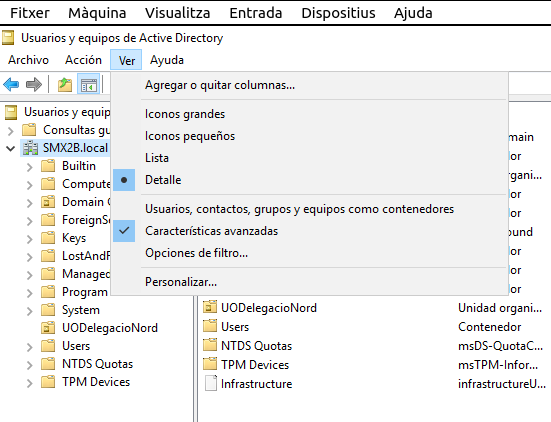
\includegraphics{png/dsaCarateristicasAvanzadas.png}
\caption{\emph{Figura 9: Veure-ho tot en dsa.msc}}
\end{figure}

\begin{itemize}
\tightlist
\item
  Ara ja apareix la pestanya \emph{Propiedades\textgreater Objeto} en
  per desprotegir (convindria que la tornàreu a deixar com estava en
  acabar).
\end{itemize}

\begin{figure}
\centering
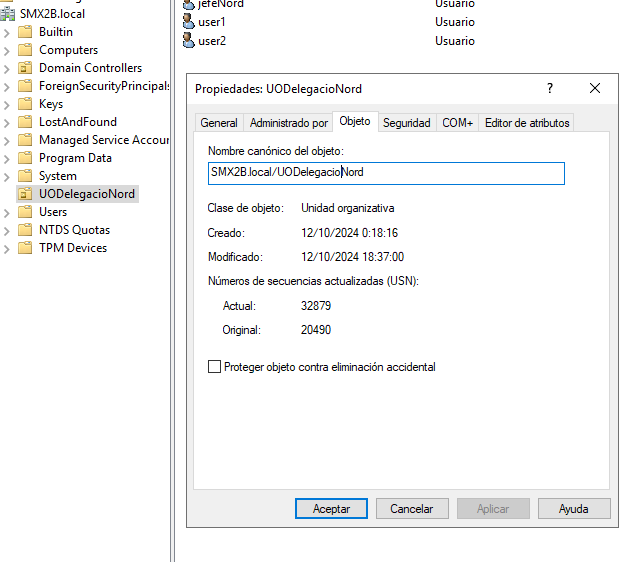
\includegraphics{png/protegerUO.png}
\caption{\emph{Figura 10: Desprotegir temporalment les UO}}
\end{figure}

\begin{itemize}
\tightlist
\item
  També ens apareix la pestanya \emph{Propiedades\textgreater Seguridad}
  on podem veure quin usuari té el control.
\end{itemize}

\begin{figure}
\centering
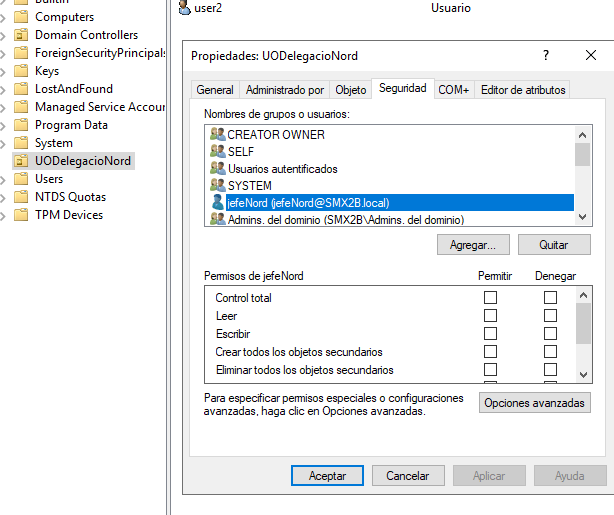
\includegraphics{png/seguridaddeUO.png}
\caption{\emph{Figura 11: Qui té el control de la UO}}
\end{figure}

\begin{itemize}
\tightlist
\item
  Entrem en \emph{Características Avanzadas} i veiem tot la informació
  detallada sobre quins usuaris i quis drets tenen sobre la UO. Des
  d'ací podem afegir i llevar usuaris i drets.
\end{itemize}

\begin{figure}
\centering
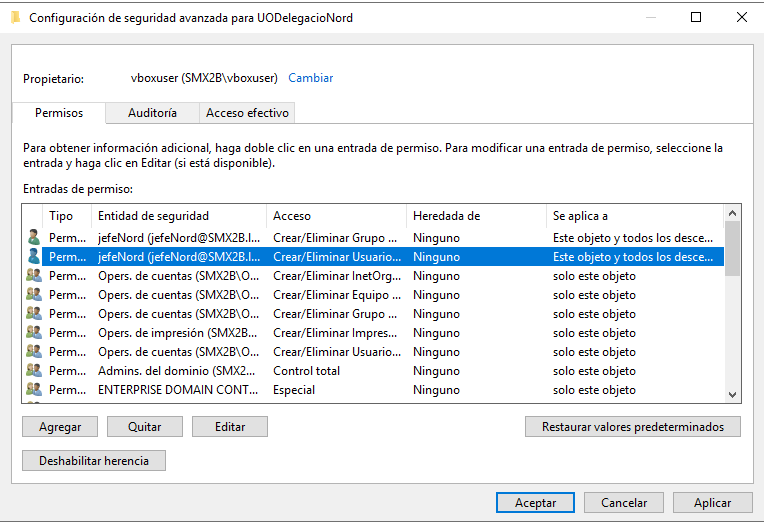
\includegraphics{png/derechosUOAvanzado.png}
\caption{*Figura 12: Gestió de drets i usuaris sobre la UO}
\end{figure}

\end{document}
